\documentclass{beamer}


\usepackage{listings}
\usepackage[italian]{babel}
\usepackage[T1]{fontenc}
\usepackage{beamerthemebjeldbak}
\usepackage{graphicx}
\usepackage{listings}
\usepackage[utf8]{inputenc} 
\usepackage{epsfig}  
\usepackage{amsmath} 
\usepackage{multicol}
\usepackage{amsfonts}
\usepackage{hyperref}

\usepackage{listings}% http://ctan.org/pkg/listings
\lstset{
  basicstyle=\ttfamily,
  mathescape
}

\setbeamertemplate{itemize/enumerate body begin}{\footnotesize}

\title{Big Network Visualizzation Tool for iNSIdEnano}
\author{Luigi Giugliano$^1$, Marco Mecchia$^1$}
\institute{$^1$Universit\'a degli studi di Salerno}


\begin{document}

\begin{frame}
   \maketitle
\end{frame}

\begin{frame}
  \frametitle{Overview}
  \footnotesize \tableofcontents
\end{frame}

\AtBeginSection[]
  {
     \begin{frame}<beamer>
     \frametitle{Overview}
   \footnotesize \tableofcontents[currentsection]
     \end{frame}
}


\section{iNSIdEnano}
\subsection{Dati}
\begin{frame}
\frametitle{iNSIdEnano}
iNSIdEnano è un tool grafico che mette in evidenza le connessioni tra entità fenotipiche del tipo:
\begin{itemize}
\item Esposizione ai nanomateriali
\item Trattamenti farmaceutici
\item Esposizione ad agenti chimici
\item Malattie
\end{itemize}
L' interazione tra queste entità è valutata in base al loro effetto sull'espressione dei geni.
\end{frame}

\begin{frame}
\begin{center}
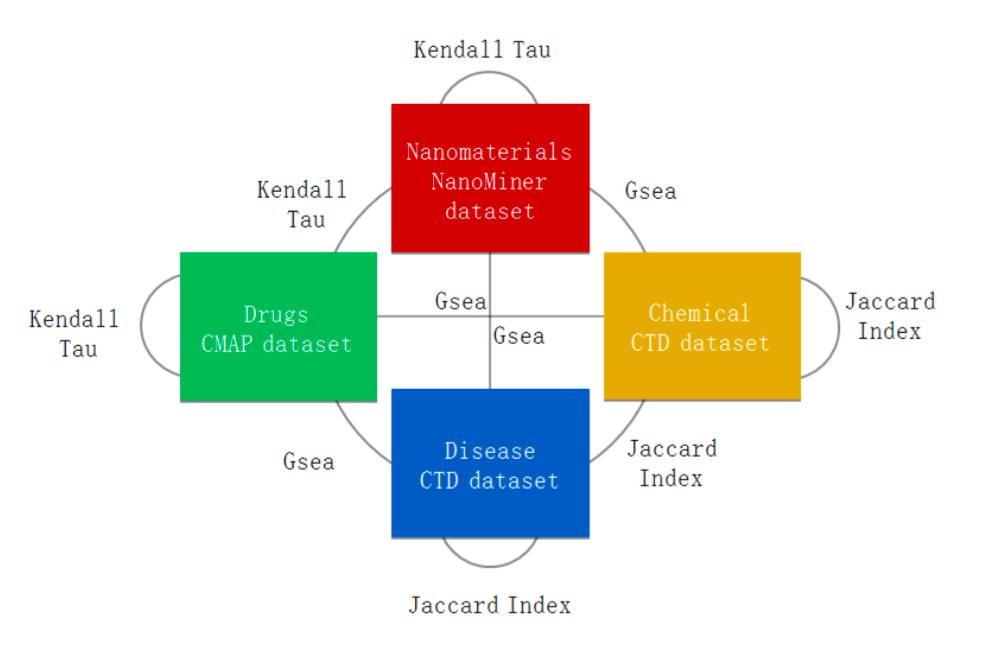
\includegraphics[scale=0.27]{img/OverviewGraph.png}
\end{center}
E' stata calcolata la distanza per ogni coppia di entità. Sono poi state normalizzate tra -1 e 1 per renderle confrontabili.
\end{frame}

\begin{frame}
Per ogni entità fenotipica nel dataset, è assegnata una lista di geni. In particolare un'insieme di geni è associato a ogni malattia e ogni agente chimico, invece per ogni farmaco e per ogni nanomateriale è associata una lista ordinata di geni. \\
\medskip
Quindi per costruire una network di similarità tra entità fenotipiche è stato necessario calcolare la similarità a coppie per ogni entità.
\end{frame}

\subsection{Generazione Network}
\begin{frame}
\frametitle{Insieme di geni vs Insieme di geni}
Il Jaccard index è stato utilizzato per calcolare la similarità tra due malattie, tra due agenti chimici o tra un agente chimico e una malattia.\\
Dati due insiemi A e B l'indice di Jaccard è dato dalla dimensione della loro intersezione diviso la dimensione della loro unione.
\begin{equation}
J(A, B) = \frac{|A \cap B|}{|A \cup  B|}
\end{equation}
Questa misura è zero se i due insieme non condividono neanche un gene, mentre 1 se sono esattamente uguali.\\
Per ogni agente chimico vengono considerati due set di geni: quelli che sono up-regolati da quell'agente chimico e quelli che sono down-regolati.
Per quelli down-regolati il Jaccard index è calcolato con il segno negativo.
\end{frame}


\begin{frame}
\frametitle{Geni ordinati vs Geni ordinati}
La distanza Kendall Tau è stata utilizzata per calcolare la similarità tra nanomateriali e nanomateriali, tra farmaci e farmaci e tra nanomateriali e farmaci, basata sulla lista ordinata dei geni.
La distanza Kendall Tau tra due liste $T1$ e $T2$ è definita come segue:
\begin{equation}
K(T_1, T_2) = |(i, j): i < j, (T_1(i) < T_1(i) \wedge  T_2(i) > T_2(j)) \vee
\end{equation}
\begin{center}$
 (T_1(i) > T_i(j) \wedge T_2(i) < T_2(J))  |
$
\end{center}
questa distanza è compresa tra 0 e $n(n$ $1)$, dove $n$ è la lunghezza della lista. Il valore significa che gli elementi nella lista sono nello stesso ordine, mentre il valore $n(n$ $1)$, indica che gli elementi sono in ordine opposto
\end{frame}

\begin{frame}
\frametitle{Genio ordinati vs insieme di geni}
La Gen Set Enrichment Analysis (GSEA), basata sul test di Kolmogorov-Smirnov, è stato usata per calcolare la similarità a coppie tra nanomateriali e malattie, tra nanomateriali e agenti chimici, tra farmaci e malattie ed infine tra farmaci e agenti chimici. Il test di KolmogorovSmirnov può essere usato per confrontare elementi con una distribuzione di probabilità. La distribuzione empirica $F_n$ per osservazioni \textit{iid}, è definito:
\begin{equation}
F_n(x) = \frac{1}{n} \sum\limits_{i=1}^n I[-\inf,x](x_i)
\end{equation}
\end{frame}

\begin{frame}
dove:
\begin{center}
$I[-\inf,x](x_i)$
\end{center}
è la funzione definita su $X$ che indica l'appartenenza di un elemento in un sottoinsieme $A$ di $X$ che ha valore 1 per tutti gli elementi di $A$ e 0 per tutti gli elementi di $X$ non in $A$. La statistica KolmogorovSmirnov per una distribuzione cumulativa $F(x)$ è 
\begin{center}
$D_n = sup_x[F_n(x)- F(x)]$
\end{center}
La statistica KolmogorovSmirnov è stata usata non in valore assoluto per preservare il segno. Ciò aiuta a capire se un gene è up o down-regolato, ovviamente anche questi valori sono stati normalizzati tra $[-1:1]$
\end{frame}

\subsection{Implmentazione}
\begin{frame}
\frametitle{Implmentazione}
INSIdEnano è stato implemetato in $R$ usando Shiny come libreria per l'interfaccia grafica. Il sistema è stato implementato in una struttura client-server: il client è responsabile per la gestione dell'interfaccia, mentre il serve processa i dati dal database in base agli input dell'utente,  e restituisce il risultato di tale computazione al client.
\end{frame}


\section{Problema}
\begin{frame}
Parliamo ora della mole di questi dati,\\
i nodi presenti in questo grafo sono: 3686
per quanto riguarda gli archi la situazione risulta essere molto più complessa, perché come spiegato precedente sono state calcolate le distanze tra tutte le coppie. e quindi il grafo senza sogliature ha  \textasciitilde 15 000 000 archi.
Il che rende questo grafo:\\
\begin{center}
\textbf{INVISUALIZZABILE}
\end{center}
\end{frame}

\begin{frame}
METTERE IMMAGINE GRAFICO INVISUALIZZABILE
\end{frame}

\section{Soluzione}
\subsection{Idea}
\begin{frame}
\frametitle{Idea}
La nostra idea consiste nel creare una visualizzazione esplorativa, di tale network. Partendo da un piccolo sottoinsieme di informazioni. E guidati dall'input dell'utente in maniera incrementale aggiungere il minor numero di informazioni alla network per aiutare l'utente nella scelta del prossimo nodo di cui avere informazioni.\\
\medskip
In questo modo le informazioni visualizzate sono quelle che l'utente ha richiesto e non tutte quelle presenti nella network. Parlando in termini di grafo in questo modo verranno visualizzati solo gli archi incidenti ai nodi scelti dall'utente. 
\end{frame}

\begin{frame}
L'idea spiegata precedentemente risulta realizzabile perché la sia per quanto riguarda gli agenti chimici che per i farmaci esistono delle gerarchie.
Ovvero ogni elemento di queste due classi appartiene ad una supercasse, che rappresenta le caratteristiche generiche degli elementi che ne fanno parte. Esempio:\\
\medskip
\begin{center}
''Organic Chemicals :- Dichlorophen''\\
''Enzymes and Coenzymes :- Neopterin''
\end{center}
Tale gerarchia può essere aumentata con ulteriori livelli. Nel nostro caso però ci siamo fermati a un livello.
\end{frame}

\begin{frame}
Però per quanto riguarda i nanomateriali e le malattie tali gerarchie non sono presenti. Il problema però non si pone per i nanomateriali perché essendo solo 29 risultano facilmente visualizzabili.\\
\medskip
Per le malattie il discorso è leggermente diverso essendo, circa 600 si sconsiglia di scegliere tale categoria per l'inizio dell'esplorazione
\end{frame}

\subsection{Realizzazione}
\begin{frame}
L'idea iniziale è quella di visualizzare solo le 4 macro-categorie:\\
INSERIRE IMMAGINE
\end{frame}

\begin{frame}
una volta scelta una categoria da cui partire l'esplorazione è possibile espanderla (doppio click) e visualizzare solo le sue sotto-categorie (se presenti).\\
INSERIRE IMMAGINE
\end{frame}

\begin{frame}
Scelta una sotto-categoria è possibile espanderla per visualizzare i veri nodi e le connessione tra di essi.\\
INSERIRE IMMAGINE 
\end{frame}

\begin{frame}
Una volta ripetuta questa operazione su di un'altra macro-categoria e successivamente su di una sua  sotto-categoria.\\
INSERIRE IMMAGINE
\end{frame}

\begin{frame}
E' possibile con (Alt + click) visualizzare gli archi che escono da quel nodo e che entrano in uno che fa parte di un'altra macro-categoria.\\
INSERIRE IMMAGINE
\end{frame}

\begin{frame}
Ricliccando un di un nodo che rappresenta una sotto-categoria o uno che rappresenta la macro-categoria i nodi che erano precedente espansi vengono eliminati e si torna ad una stato iniziale.\\
\medskip
La stessa cosa vale per le informazioni aggiunge attraverso alt + click, anche esse possono essere rimosse ricliccando sullo stesso nodo. 
\end{frame}

\begin{frame}
Un'altra feature che è stata inserita per facilitare la visualizzazione è quella dello Shift + click. Che cliccato su di un nodo mette in evidenza tutti gli archi incidenti su quel nodo e i nodi che fanno parte del vicinato di quel nodo, nascondendo tutti gli altri.\\
INSERIRE IMMAGINE.
\end{frame}


\begin{frame}
Inoltre sono state aggiunte una serie di features accessorie che semplificano la visualizzazione come:
\begin{itemize}
\item Colorazione degli archi in base al valore (verdi: positivi, rossi: negativi)
\item Spessore degli archi in base al valore
\item Legenda in alto a sinistra per i nodi, a destra per gli archi
\item Label su gli archi
\item Label sui nodi.
\item Drag and drop, release.
\end{itemize}
\end{frame}

\begin{frame}
INSERIRE LE IMMAGINI DELLA LISTA DI PRIMA
\end{frame}

\subsection{Implementazione}
\begin{frame}
\frametitle{Implementazione}
Il core dell'implementazione è stata effettuata in Javascript, attraverso una libreria di visualizzazione  di grafi chiamata:
\begin{center}
\href{http://d3js.org/}{d3.js}
\end{center}
che si collega ad R attraverso un ''HTMLWidgets'' che può essere renderizzato all'interno di uno shiny widget oppure chiamato come visualizzatore di dati R generico.
\end{frame}

\begin{frame}
E' stato creato il package R che è possibile installare su qualsiasi ambiente avente la versione di R maggiore di 3.2, per motivi di compatibilità.\\
E' possibile trovare tale pacchetto al link:
\begin{center}
\url{https://github.com/Abelarm/BioInf_Project}
\end{center}
\end{frame}

\section{Bonus}
\begin{frame}
\frametitle{Bonus}
Sulla stessa falsa riga, è stato creato un'ulteriore tool per la visualizzazione di un grafo diverso, ma sfruttando le stesse idee. Però il grafo non è quello completo, ma bensì la network che risulta dalla clustering in base ai nanomateriali.\\
\medskip
Dove per ogni nanomateriale vi sono solo i collegamenti con gli elementi facenti parti delle altre 3 macro-categorie.
\end{frame}

\begin{frame}
INSERIRE IMMAGINE GRAFO DI MERDA
\end{frame}

\begin{frame}
INSERIRE VARIE IMMAGINI DEL NOSTRO GRAFO
\end{frame}

\end{document}